
\includegraphics[width=8.49444in,height=4.14861in]{12-RDM/Cours/pandoc/media/image1.png}

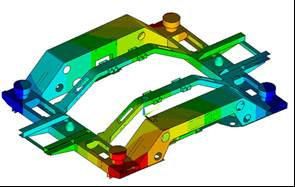
\includegraphics[width=4.25884in,height=2.69697in]{12-RDM/Cours/pandoc/media/image3.jpeg}

Cycle 7 : Dimensionner les pièces d'un mécanisme

\textbf{Résistance des matériaux}

Thomas Lusseau

Lycée Robert Doisneau - ATS

\hypertarget{table-des-matiuxe8res}{%
\section*{Table des matières}\label{table-des-matiuxe8res}}
\addcontentsline{toc}{section}{Table des matières}

\protect\hyperlink{besoin-rempli-par-la-ruxe9sistance-des-matuxe9riaux}{1. Besoin rempli par la résistance des matériaux {[}5{]}(\#besoin-rempli-par-la-résistance-des-matériaux)}

\protect\hyperlink{hypothuxe8ses-de-la-ruxe9sistance-des-matuxe9riaux}{2. Hypothèses de la résistance des matériaux {[}5{]}(\#hypothèses-de-la-résistance-des-matériaux)}

\protect\hyperlink{thuxe9orie-des-poutres-droites}{2.1. Théorie des poutres droites {[}5{]}(\#théorie-des-poutres-droites)}

\protect\hyperlink{matuxe9riaux-de-construction}{2.2. Matériaux de construction {[}6{]}(\#matériaux-de-construction)}

\protect\hyperlink{efforts-invariants}{2.3. Efforts invariants {[}6{]}(\#efforts-invariants)}

\protect\hyperlink{hypothuxe8se-de-barruxe9-de-saint-venant}{2.4. Hypothèse de Barré de Saint-Venant {[}6{]}(\#hypothèse-de-barré-de-saint-venant)}

\protect\hyperlink{hypothuxe8se-de-navier-bernoulli}{2.5. Hypothèse de Navier-Bernoulli {[}7{]}(\#hypothèse-de-navier-bernoulli)}

\protect\hyperlink{principe-de-superposition-de-linuxe9arituxe9}{2.6. Principe de superposition (de linéarité) {[}7{]}(\#principe-de-superposition-de-linéarité)}

\protect\hyperlink{moduxe9lisation-des-actions-muxe9caniques-extuxe9rieures}{3. Modélisation des actions mécaniques extérieures {[}7{]}(\#modélisation-des-actions-mécaniques-extérieures)}

\protect\hyperlink{actions-muxe9caniques-extuxe9rieures}{3.1. Actions mécaniques extérieures {[}7{]}(\#actions-mécaniques-extérieures)}

\protect\hyperlink{les-liaisons}{3.2. Les liaisons {[}8{]}(\#les-liaisons)}

\protect\hyperlink{actions-muxe9caniques-intuxe9rieures-torseur-de-cohuxe9sion}{4. Actions mécaniques intérieures (torseur de cohésion) {[}8{]}(\#actions-mécaniques-intérieures-torseur-de-cohésion)}

\protect\hyperlink{coupure-dans-une-poutre}{4.1. Coupure dans une poutre {[}8{]}(\#coupure-dans-une-poutre)}

\protect\hyperlink{duxe9termination-du-torseur-de-cohuxe9sion}{4.2. Détermination du torseur de cohésion {[}9{]}(\#détermination-du-torseur-de-cohésion)}

\protect\hyperlink{nature-des-sollicitations}{4.3. Nature des sollicitations {[}10{]}(\#nature-des-sollicitations)}

\protect\hyperlink{traction}{5. Traction {[}11{]}(\#traction)}

\protect\hyperlink{duxe9finition}{5.1. Définition {[}11{]}(\#définition)}

\protect\hyperlink{contrainte-normale}{5.2. Contrainte normale {[}12{]}(\#contrainte-normale)}

\protect\hyperlink{condition-de-ruxe9sistance}{5.3. Condition de résistance {[}12{]}(\#condition-de-résistance)}

\protect\hyperlink{flexion}{6. Flexion {[}13{]}(\#flexion)}

\protect\hyperlink{condition-de-ruxe9sistance-1}{6.1. Condition de résistance {[}14{]}(\#condition-de-résistance-1)}

\protect\hyperlink{duxe9formations}{6.2. Déformations {[}14{]}(\#déformations)}

\protect\hyperlink{sources}{7. Sources {[}14{]}(\#sources)}

\protect\hyperlink{exercices-du-chapitre}{8. Exercices du chapitre {[}15{]}(\#exercices-du-chapitre)}

Définir les notions de poutre et les hypothèses fondamentales de la résistance des matériaux

Identifier et caractériser les sollicitations simples.

Je connais~:

\begin{longtable}[]{@{}
  >{\raggedright\arraybackslash}p{(\columnwidth - 2\tabcolsep) * \real{0.9306}}
  >{\raggedright\arraybackslash}p{(\columnwidth - 2\tabcolsep) * \real{0.0556}}@{}}
\toprule\noalign{}
\begin{minipage}[b]{\linewidth}\raggedright
\begin{itemize}
\tightlist
\item
  Les principales sollicitations~: flexion simple, torsion simple, traction--compression
\end{itemize}
\end{minipage} & \begin{minipage}[b]{\linewidth}\raggedright
⃝
\end{minipage} \\
\midrule\noalign{}
\endhead
\bottomrule\noalign{}
\endlastfoot
\begin{minipage}[t]{\linewidth}\raggedright
\begin{itemize}
\tightlist
\item
  L'expression des contraintes et déformations
\end{itemize}
\end{minipage} & ⃝ \\
\begin{minipage}[t]{\linewidth}\raggedright
\begin{itemize}
\tightlist
\item
  Le torseur de cohésion
\end{itemize}
\end{minipage} & ⃝ \\
\begin{minipage}[t]{\linewidth}\raggedright
\begin{itemize}
\tightlist
\item
  Les notions coefficient de sécurité et résistance mécanique
\end{itemize}
\end{minipage} & ⃝ \\
\end{longtable}

Je sais~:

\begin{longtable}[]{@{}
  >{\raggedright\arraybackslash}p{(\columnwidth - 2\tabcolsep) * \real{0.9306}}
  >{\raggedright\arraybackslash}p{(\columnwidth - 2\tabcolsep) * \real{0.0556}}@{}}
\toprule\noalign{}
\begin{minipage}[b]{\linewidth}\raggedright
\begin{itemize}
\tightlist
\item
  Poser les hypothèses nécessaires à une étude de RdM (Poutre, Navier-Bernoulli, \ldots)
\end{itemize}
\end{minipage} & \begin{minipage}[b]{\linewidth}\raggedright
⃝
\end{minipage} \\
\midrule\noalign{}
\endhead
\bottomrule\noalign{}
\endlastfoot
\begin{minipage}[t]{\linewidth}\raggedright
\begin{itemize}
\tightlist
\item
  Identifier les contraintes, les déformations et les sollicitations d'un solide
\end{itemize}
\end{minipage} & ⃝ \\
\begin{minipage}[t]{\linewidth}\raggedright
\begin{itemize}
\tightlist
\item
  Choisir un modèle de solide (indéformable ou déformable) en fonction de l'objectif visé
\end{itemize}
\end{minipage} & ⃝ \\
\begin{minipage}[t]{\linewidth}\raggedright
\begin{itemize}
\tightlist
\item
  Déterminer le torseur de cohésion dans un solide
\end{itemize}
\end{minipage} & ⃝ \\
\begin{minipage}[t]{\linewidth}\raggedright
\begin{itemize}
\tightlist
\item
  Associer un modèle de contraintes à l'état de sollicitation
\end{itemize}
\end{minipage} & ⃝ \\
\begin{minipage}[t]{\linewidth}\raggedright
\begin{itemize}
\tightlist
\item
  Proposer ou justifier des conditions aux limites dans un logiciel de simulation par éléments finis
\end{itemize}
\end{minipage} & ⃝ \\
\begin{minipage}[t]{\linewidth}\raggedright
\begin{itemize}
\tightlist
\item
  Déterminer la répartition des contraintes dans une section droite
\end{itemize}
\end{minipage} & ⃝ \\
\begin{minipage}[t]{\linewidth}\raggedright
\begin{itemize}
\tightlist
\item
  Vérifier la résistance mécanique d'une poutre droite
\end{itemize}
\end{minipage} & ⃝ \\
\begin{minipage}[t]{\linewidth}\raggedright
\begin{itemize}
\tightlist
\item
  Déterminer le coefficient de sécurité par rapport aux exigences du cahier des charges fonctionnel
\end{itemize}
\end{minipage} & ⃝ \\
\begin{minipage}[t]{\linewidth}\raggedright
\begin{itemize}
\tightlist
\item
  Déterminer l'équation de la flèche dans une poutre droite soumise à de la flexion, avec chargements ponctuels ou répartition linéique constante de pression
\end{itemize}
\end{minipage} & ⃝ \\
\end{longtable}

\hypertarget{besoin-rempli-par-la-ruxe9sistance-des-matuxe9riaux}{%
\subsection{Besoin rempli par la résistance des matériaux}\label{besoin-rempli-par-la-ruxe9sistance-des-matuxe9riaux}}

La statique étudie l'équilibre des systèmes de solides, supposés indéformables. La réalité montre que cette hypothèse fondamentale est très restrictive et ne peut que rarement être correctement validée. De plus, certains problèmes de statique (notion d'hyperstatisme) n'ont été résolus que partiellement.

On introduit donc une nouvelle théorie, la Résistance des Matériaux (RdM), qui permettra l'étude de solides déformables, à la condition qu'ils soient modélisables par un élément longiligne : la poutre.

La RdM permet d'étudier les relations déformations-actions extérieures dans les solides longilignes. La RdM permet aussi de calculer ou de vérifier le dimensionnement des éléments d'un système mécanique et de choisir le matériau à travers certains paramètres le caractérisant.

\begin{longtable}[]{@{}
  >{\raggedright\arraybackslash}p{(\columnwidth - 4\tabcolsep) * \real{0.3284}}
  >{\raggedright\arraybackslash}p{(\columnwidth - 4\tabcolsep) * \real{0.3284}}
  >{\raggedright\arraybackslash}p{(\columnwidth - 4\tabcolsep) * \real{0.3284}}@{}}
\toprule\noalign{}
\begin{minipage}[b]{\linewidth}\raggedright
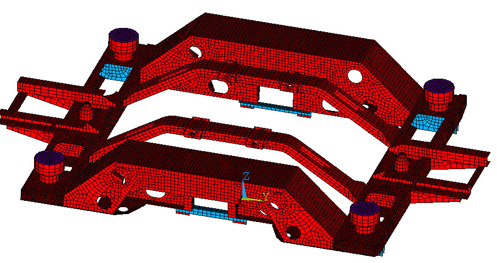
\includegraphics{12-RDM/Cours/pandoc/media/image5.png}
\end{minipage} & \begin{minipage}[b]{\linewidth}\raggedright
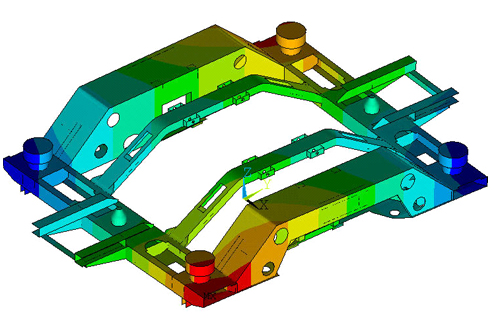
\includegraphics{12-RDM/Cours/pandoc/media/image6.png}
\end{minipage} & \begin{minipage}[b]{\linewidth}\raggedright
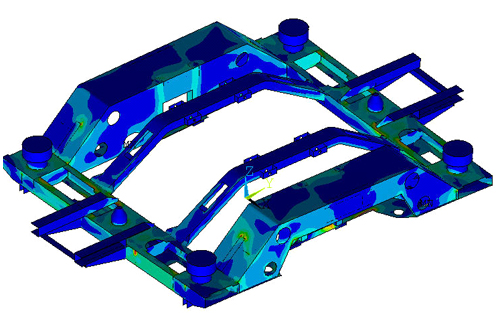
\includegraphics{12-RDM/Cours/pandoc/media/image7.png}
\end{minipage} \\
\midrule\noalign{}
\endhead
\bottomrule\noalign{}
\endlastfoot
Géométrie et maillage & Déplacements & Contraintes \\
\end{longtable}

Etude d'un bissel (essieu porteur orientable par rapport au châssis) de wagon

\hypertarget{hypothuxe8ses-de-la-ruxe9sistance-des-matuxe9riaux}{%
\subsection{Hypothèses de la résistance des matériaux}\label{hypothuxe8ses-de-la-ruxe9sistance-des-matuxe9riaux}}

\hypertarget{thuxe9orie-des-poutres-droites}{%
\subsubsection{Théorie des poutres droites}\label{thuxe9orie-des-poutres-droites}}


\includegraphics{12-RDM/Cours/pandoc/media/image8.wmf}Les notions abordées dans ce cours ne sont valables que pour des solides ayant une forme de \textbf{poutre}, c'est-à-dire un solide pour lequel :

\begin{itemize}
\item
  Il existe une \textbf{ligne moyenne}, continue, passant par les barycentres des sections du solide
\item
  La longueur L est au moins 4 à 5 fois supérieure au diamètre D
\item
  Il n'y a pas de brusque variation de section (trous, épaulements)
\item
  Le solide admet un seul et même \textbf{plan de symétrie pour les charges et la géométrie}
\end{itemize}

\ul{Remarque}

Dans le cas d'un solide constitué de plusieurs poutres droites, il suffit de décomposer l'étude en autant d'études que de tronçons rectilignes.

\hypertarget{matuxe9riaux-de-construction}{%
\subsubsection{Matériaux de construction}\label{matuxe9riaux-de-construction}}

On suppose que les matériaux de construction possèdent les propriétés suivantes :

Ils sont \textbf{homogènes}, la constitution est la même en chaque point

Ils sont \textbf{isotropes}, leurs propriétés physiques sont identiques dans toutes les directions. L\textquotesingle isotropie est vérifiée pour les aciers non fibrés (les aciers laminés et forgés ne sont pas isotropes). Cette hypothèse n\textquotesingle est pas vérifiée pour le bois, les matériaux composites, etc.

Ils sont \textbf{continus}, c'est à dire que les discontinuités microscopiques sont négligées

Ils sont \textbf{élastiques} et \textbf{linéaires}

\hypertarget{efforts-invariants}{%
\subsubsection[Efforts invariants]{\texorpdfstring{\protect
\includegraphics[width=3.34861in,height=1.96875in]{12-RDM/Cours/pandoc/media/image9.emf}Efforts invariants}{Efforts invariants}}\label{efforts-invariants}}

Les déplacements sous charges étant petits, les efforts extérieurs sont supposés invariants dans R(A,x\textsubscript{0},y\textsubscript{0},z\textsubscript{0}) repère lié à la poutre non déformée avant et après application du chargement. Ainsi, on considère que δ = 0.

La charge \(\overrightarrow{B}\) n'est pas appliquée brutalement mais progressivement. Les calculs devraient se faire dans la configuration déformée, qu'on suppose proche donc confondue avec la configuration initiale.

\hypertarget{hypothuxe8se-de-barruxe9-de-saint-venant}{%
\subsubsection{Hypothèse de Barré de Saint-Venant}\label{hypothuxe8se-de-barruxe9-de-saint-venant}}

L'état des \textbf{sollicitations} (dans la section droite de centre G) dans une région suffisamment \textbf{éloignée des points d'applications des charges extérieures} appliquées à la poutre ne dépend que du torseur associé à ces charges. Par éloigné, il faut entendre une distance au moins égale à la plus grande dimension de la section transversale de la poutre.

\begin{longtable}[]{@{}
  >{\raggedright\arraybackslash}p{(\columnwidth - 4\tabcolsep) * \real{0.4865}}
  >{\raggedright\arraybackslash}p{(\columnwidth - 4\tabcolsep) * \real{0.0541}}
  >{\raggedright\arraybackslash}p{(\columnwidth - 4\tabcolsep) * \real{0.4459}}@{}}
\toprule\noalign{}
\begin{minipage}[b]{\linewidth}\raggedright

\includegraphics[width=2.80189in,height=1.06205in]{1 2-RDM/Cours/pandoc/media/image10. emf}
\end{minipage} & \begin{minipage}[b]{\linewidth}\raggedright
1 .
\end{minipage} & \begin{minipage}[b]{\linewidth}\raggedright

\includegraphics[width=3.14905in,height=0.90566in]{12-RDM/ Cours/pandoc/media/image10.emf}
\end{minipage} \\
\midrule\noalign{}
\endhead
\bottomrule\noalign{}
\endlastfoot
\textsubscript{cas~a}\{τ\textsubscript{(S1→S1}\}\textsubscript{G} & = & \textsubscript{cas~b}\{τ\textsubscript{(S1→S1)}\}\textsubscript{G} \\
\end{longtable}

\hypertarget{hypothuxe8se-de-navier-bernoulli}{%
\subsubsection[Hypothèse de Navier-Bernoulli]{\texorpdfstring{\protect
\includegraphics[width=3.22639in,height=1.79236in]{12-RDM/Cours/pandoc/media/image11.emf}Hypothèse de Navier-Bernoulli}{Hypothèse de Navier-Bernoulli}}\label{hypothuxe8se-de-navier-bernoulli}}

Les sections planes, normales à la ligne moyenne avant chargement demeurent planes et normales à la ligne moyenne après chargement~: \textbf{pas de gauchissement (distorsion) des sections droites}

Cette hypothèse s'applique bien aux poutres élancées fléchies, ainsi qu'à l'étude des sollicitations de traction, compression, torsion des poutres de section circulaire flexion pure...

Elle est mise en défaut pour des poutres de section non circulaire, sollicitées en torsion, et pour des poutres courtes sollicitées en flexion.

\hypertarget{principe-de-superposition-de-linuxe9arituxe9}{%
\subsubsection{Principe de superposition (de linéarité)}\label{principe-de-superposition-de-linuxe9arituxe9}}

Les relations actions mécaniques extérieures / réactions aux appuis, responsables des déformations sont supposées linéaires.

L'effet mécanique dû à un ensemble d'actions mécaniques agissant sur une poutre dans son domaine élastique est égal à la somme des effets produits par chaque action mécanique prise séparément.


\includegraphics[width=6.33962in,height=1.45751in]{12-RDM/Cours/pandoc/media/image12.emf}

\hypertarget{moduxe9lisation-des-actions-muxe9caniques-extuxe9rieures}{%
\subsection{Modélisation des actions mécaniques extérieures}\label{moduxe9lisation-des-actions-muxe9caniques-extuxe9rieures}}

\hypertarget{actions-muxe9caniques-extuxe9rieures}{%
\subsubsection{Actions mécaniques extérieures}\label{actions-muxe9caniques-extuxe9rieures}}

La modélisation du solide par une poutre implique le passage d'un espace tridimensionnel à un espace unidimensionnel.

De la même façon, la modélisation des actions mécaniques extérieures à la poutre résulte d'une transposition d'un problème tridimensionnel à un problème unidimensionnel.

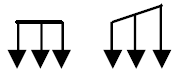
\includegraphics[width=0.98056in,height=0.42014in]{12-RDM/Cours/pandoc/media/image13.png}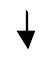
\includegraphics[width=0.33019in,height=0.40322in]{12-RDM/Cours/pandoc/media/image14.png}Les actions mécaniques extérieures agissant sur la poutre pourront se présenter sous la forme de glisseurs ou de couples, concentrés (vecteurs liés) ou répartis (charge volumique, surfacique ou linéique).

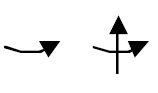
\includegraphics[width=0.46736in,height=0.29236in]{12-RDM/Cours/pandoc/media/image15.png}

\ul{Remarque}

Un système d'actions mécaniques extérieures ne peut plus être remplacé par un système d'actions mécaniques extérieures équivalent comme c'était le cas en statique.


\includegraphics[width=4.82075in,height=0.83003in]{12-RDM/Cours/pandoc/media/image16.emf}

\hypertarget{les-liaisons}{%
\subsubsection{Les liaisons}\label{les-liaisons}}

La poutre est reliée au bâti par des liaisons qui induisent une suppression des certains déplacements. Ces conditions de déplacement (en translation ou en rotation) permettent d'apporter des renseignements supplémentaires pour la résolution des problèmes.

\begin{longtable}[]{@{}
  >{\raggedright\arraybackslash}p{(\columnwidth - 6\tabcolsep) * \real{0.2639}}
  >{\raggedright\arraybackslash}p{(\columnwidth - 6\tabcolsep) * \real{0.2500}}
  >{\raggedright\arraybackslash}p{(\columnwidth - 6\tabcolsep) * \real{0.2222}}
  >{\raggedright\arraybackslash}p{(\columnwidth - 6\tabcolsep) * \real{0.2361}}@{}}
\toprule\noalign{}
\begin{minipage}[b]{\linewidth}\raggedright
\begin{enumerate}
\def\labelenumi{\arabic{enumi}.}
\setcounter{enumi}{1}
\tightlist
\item
  
\includegraphics{12 -RDM/Cours/pando c/media/image17. png}\{width=``0.62 2642169728784in''
\end{enumerate}

height=``0.6944 860017497813in''\}
\end{minipage} & \begin{minipage}[b]{\linewidth}\raggedright
\begin{enumerate}
\def\labelenumi{\arabic{enumi}.}
\setcounter{enumi}{2}
\tightlist
\item
  
\includegraphics{12-RDM/ Cours/pandoc/me dia/image18.png}\{width=``0.5941 010498687664in''
\end{enumerate}

height=``0.5471 69728783902in''\}
\end{minipage} & \begin{minipage}[b]{\linewidth}\raggedright
\begin{enumerate}
\def\labelenumi{\arabic{enumi}.}
\setcounter{enumi}{3}
\tightlist
\item
  \includegraphics{12 -RDM/Cours/pa ndoc/media/im age19.png}\{wi dth=``0.539621 6097987752in'' heig ht=``0.4905653 980752406in''\}
\end{enumerate}
\end{minipage} & \begin{minipage}[b]{\linewidth}\raggedright
\begin{enumerate}
\def\labelenumi{\arabic{enumi}.}
\setcounter{enumi}{4}
\tightlist
\item
  ! \href{12-RDM/Cour\%20s/pandoc/media\%20/image20.png}{}\{ width=``0.68263 12335958006in'' he ight=``0.622641 0761154856in''\}
\end{enumerate}
\end{minipage} \\
\midrule\noalign{}
\endhead
\bottomrule\noalign{}
\endlastfoot
\begin{minipage}[t]{\linewidth}\raggedright
\begin{enumerate}
\def\labelenumi{\arabic{enumi}.}
\setcounter{enumi}{5}
\tightlist
\item
  \emph{\ul{Liaison encastreme nt}}
\end{enumerate}
\end{minipage} & \begin{minipage}[t]{\linewidth}\raggedright
\begin{enumerate}
\def\labelenumi{\arabic{enumi}.}
\setcounter{enumi}{6}
\tightlist
\item
  \emph{\ul{Liaison rotule (appui fixe )}}
\end{enumerate}
\end{minipage} & \begin{minipage}[t]{\linewidth}\raggedright
\begin{enumerate}
\def\labelenumi{\arabic{enumi}.}
\setcounter{enumi}{7}
\tightlist
\item
  \emph{{[}Liaison pivot (a rticulation){]} \{.underline\}}
\end{enumerate}
\end{minipage} & \begin{minipage}[t]{\linewidth}\raggedright
\begin{enumerate}
\def\labelenumi{\arabic{enumi}.}
\setcounter{enumi}{8}
\tightlist
\item
  \emph{\ul{Liaison sphère cylindre (appui simple)}}
\end{enumerate}
\end{minipage} \\
\end{longtable}

\hypertarget{actions-muxe9caniques-intuxe9rieures-torseur-de-cohuxe9sion}{%
\subsection[Actions mécaniques intérieures (torseur de cohésion)]{\texorpdfstring{\protect
\includegraphics{12-RDM/Cours/pandoc/media/image21.wmf}Actions mécaniques intérieures (torseur de cohésion)}{Actions mécaniques intérieures (torseur de cohésion)}}\label{actions-muxe9caniques-intuxe9rieures-torseur-de-cohuxe9sion}}

\hypertarget{coupure-dans-une-poutre}{%
\subsubsection{Coupure dans une poutre}\label{coupure-dans-une-poutre}}

Considérons une poutre P, en équilibre sous l'effet d'actions mécaniques extérieures.

Pour mettre en évidence les efforts transmis par la matière au niveau de la section S, nous effectuons une \textbf{coupure imaginaire} dans un plan perpendiculaire à la ligne moyenne. Elle sépare la poutre en deux tronçons E1 et E2, tel que E = E1+E2.

Isolons le tronçon E1.

Les actions mécaniques que le tronçon E2 exerce sur le tronçon E1 à travers la section droite S sont des actions mécaniques intérieures à la poutre P.

Nous en ignorons à priori la nature, cependant la liaison entre E1 et E2 peut être modélisée par une liaison complète. On peut donc modéliser l'action mécanique E2 sur E1 par un torseur appelé :

\begin{quote}
\textbf{Torseur de cohésion\emph{~}}: 
\includegraphics{12-RDM/Cours/pandoc/media/image22.wmf} avec G sur la ligne moyenne.
\end{quote}

\ul{Vision globale~: Torseur de cohésion}

\hypertarget{duxe9termination-du-torseur-de-cohuxe9sion}{%
\subsubsection{Détermination du torseur de cohésion}\label{duxe9termination-du-torseur-de-cohuxe9sion}}

Pour ce faire, deux méthodes sont envisageables.

\ul{Isolement du tronçon \textbf{g}auche E1}

Appliquons le PFS au tronçon E1~:\(\left\{ \tau_{(\overline{E1} \rightarrow E1)} \right\} = \left\{ \tau_{(\overline{E} \rightarrow E1)} \right\} + \left\{ \tau_{(E2 \rightarrow E1)} \right\} = \left\{ 0 \right\}\)

D'où 
\includegraphics{12-RDM/Cours/pandoc/media/image23.wmf}

\ul{Isolement du tronçon \textbf{d}roit E2}

Appliquons le PFS au tronçon E2~:\(\left\{ \tau_{(\overline{E2} \rightarrow E2)} \right\} = \left\{ \tau_{(\overline{E} \rightarrow E2)} \right\} + \left\{ \tau_{(E1 \rightarrow E2)} \right\} = \left\{ 0 \right\}\)

Soit \(\left\{ \tau_{(E1 \rightarrow E2)} \right\} = \  - \left\{ \tau_{(\overline{E} \rightarrow E2)} \right\}\)

D'où 
\includegraphics{12-RDM/Cours/pandoc/media/image24.wmf}

\ul{Remarques}

\begin{itemize}
\tightlist
\item
  Différentes notations coexistent pour désigner les tronçons gauche et droite~:
\end{itemize}

Tronçon gauche = E1 (dans ce cours) = g (pour gauche) = x-

Tronçon droite = E2 (dans ce cours) = d (pour droite) = x+

Ainsi, avec la dernière notation, le torseur de cohésion s'écrira \(\left\{ T_{coh} \right\} = \left\{ T_{x + \rightarrow x -} \right\} = + \left\{ T_{ext \rightarrow x +} \right\} = - \left\{ T_{ext \rightarrow x -} \right\}\)

\begin{itemize}
\item
  Le torseur de cohésion est toujours exprimé au barycentre G de la section considérée

  \emph{\ul{Composantes du torseur de cohésion}}
\end{itemize}


\includegraphics{12-RDM/Cours/pandoc/media/image25.wmf}

\begin{quote}
N~: Effort \textbf{n}ormal sur (G,x), il est perpendiculaire à la section droite

R T\textsubscript{y}~: Effort \textbf{t}ranchant sur (G,y)

T\textsubscript{z}~: Effort \textbf{t}ranchant sur (G,z)

Mt~: Moment de \textbf{t}orsion sur (G,x), d'axe perpendiculaire à la section droite

M\textsubscript{G} Mf\textsubscript{y}~: Moment de \textbf{f}lexion sur (G,y)

Mf\textsubscript{z}~: Moment de \textbf{f}lexion sur (G,z)
\end{quote}

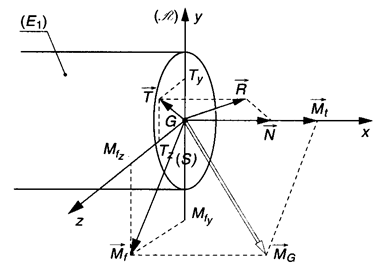
\includegraphics[width=3.42569in,height=2.39583in]{12-RDM/Cours/pandoc/media/image26.png}

\hypertarget{nature-des-sollicitations}{%
\subsubsection{Nature des sollicitations}\label{nature-des-sollicitations}}

En fonction de «~l'allure~» du torseur de cohésion, une typologie des \textbf{sollicitations} est établie.

On appelle \textbf{sollicitation simple} l\textquotesingle état de contrainte d'une poutre dont le torseur de cohésion ne comporte qu\textquotesingle un élément.

On appelle \textbf{sollicitation composée} l'état de sollicitation d'une poutre soumise à \textbf{plusieurs sollicitations simples} (par exemple~: traction + flexion pure).

\begin{longtable}[]{@{}
  >{\raggedright\arraybackslash}p{(\columnwidth - 10\tabcolsep) * \real{0.2329}}
  >{\raggedright\arraybackslash}p{(\columnwidth - 10\tabcolsep) * \real{0.0959}}
  >{\raggedright\arraybackslash}p{(\columnwidth - 10\tabcolsep) * \real{0.1370}}
  >{\raggedright\arraybackslash}p{(\columnwidth - 10\tabcolsep) * \real{0.1233}}
  >{\raggedright\arraybackslash}p{(\columnwidth - 10\tabcolsep) * \real{0.1233}}
  >{\raggedright\arraybackslash}p{(\columnwidth - 10\tabcolsep) * \real{0.2329}}@{}}
\toprule\noalign{}
\endhead
\bottomrule\noalign{}
\endlastfoot
\textbf{Nature des so llicitations} & \textbf{Ef fort Norm al} & \begin{minipage}[t]{\linewidth}\raggedright
\begin{itemize}
\tightlist
\item
  *Effort Tran chant**
\end{itemize}
\end{minipage} & \textbf{ Moment de}

\textbf{Tor sion} & \textbf{ Moment de}

\textbf{Fle xion} & \textbf{Torseur de cohésion} \\
\textbf{Traction (N\textgreater0)}

\textbf{Compression (N\textless0)} & N & T\textsubscript{y} = 0

T\textsubscript{z} = 0 & Mt=0 & Mf\textsubscript{y} = 0

Mf\textsubscript{z} = 0 & 
\includegraphics{12-RDM/Cou rs/pandoc/medi a/image27.wmf} \\
\textbf{Cisaillement simple} & N=0 & T\textsubscript{y} OU T\textsubscript{z} & Mt=0 & Mf\textsubscript{y} = 0

Mf\textsubscript{z} = 0 & 
\includegraphics{12-RDM/Cou rs/pandoc/medi a/image28.wmf} \\
\textbf{Torsion simple} & N=0 & T\textsubscript{y} = 0

T\textsubscript{z} = 0 & Mt & Mf\textsubscript{y} = 0

Mf\textsubscript{z} = 0 & 
\includegraphics{12-RDM/Cou rs/pandoc/medi a/image29.wmf} \\
\textbf{Flexion pure} & N=0 & T\textsubscript{y} = 0

T\textsubscript{z} = 0 & Mt=0 & Mf\textsubscript{y} OU Mf\textsubscript{z} & 
\includegraphics{12-RDM/Cou rs/pandoc/medi a/image30.wmf} \\
\textbf{Flexion simple} & N=0 & T\textsubscript{y} OU T\textsubscript{z} & Mt=0 & Mf\textsubscript{y} OU Mf\textsubscript{z} & 
\includegraphics{12-RDM/Cou rs/pandoc/medi a/image31.wmf} \\
\end{longtable}

\ul{Vision locale~: Contrainte en un point d'une poutre}


\includegraphics{12-RDM/Cours/pandoc/media/image32.wmf}Les efforts de cohésion, dont on connaît les éléments de réduction en G (grâce au torseur de cohésion), sont des actions mécaniques que le tronçon E2 de la poutre exerce sur le tronçon E1 à travers une section droite fictive S. La loi de répartition dans cette section S de ces efforts élémentaires est inconnue.

Regardons de plus près ce qui se passe dans cette coupure. Notons ∆f l'action mécanique élémentaire au point M et ∆S l'élément de surface entourant ce point.

Appelons n la normale extérieure en M au plan de la section S.

On appelle \textbf{vecteur contrainte} en M, relativement à la surface élémentaire ∆S, orientée par la normale extérieure n, le vecteur noté 
\includegraphics{12-RDM/Cours/pandoc/media/image33.wmf} tel que : 
\includegraphics{12-RDM/Cours/pandoc/media/image34.wmf}

On appelle \textbf{contrainte normale}
\includegraphics{12-RDM/Cours/pandoc/media/image35.wmf} la projection de 
\includegraphics{12-RDM/Cours/pandoc/media/image33.wmf} sur la normale extérieure n.

On appelle \textbf{contrainte tangentielle}
\includegraphics{12-RDM/Cours/pandoc/media/image36.wmf} la projection de 
\includegraphics{12-RDM/Cours/pandoc/media/image33.wmf} sur le plan de la facette ∆S.

Par conséquent 
\includegraphics{12-RDM/Cours/pandoc/media/image37.wmf}

Une contrainte s'exprime en Mpa = N/mm\textsuperscript{2}

\hypertarget{traction}{%
\subsection{Traction}\label{traction}}

\hypertarget{duxe9finition}{%
\subsubsection{Définition}\label{duxe9finition}}

Une poutre est sollicitée en traction lorsque les actions aux extrémités se réduisent à deux forces égales et opposées, portées par la ligne moyenne Lm.


\includegraphics{12-RDM/Cours/pandoc/media/image38.emf}

L'effort F est appelé \textbf{effort normal}, il est noté N. Quelle que soit la section considérée de la poutre, il s'exerce toujours au barycentre G de la section.


\includegraphics{12-RDM/Cours/pandoc/media/image39.emf}

\hypertarget{contrainte-normale}{%
\subsubsection{Contrainte normale}\label{contrainte-normale}}

\begin{longtable}[]{@{}
  >{\raggedright\arraybackslash}p{(\columnwidth - 2\tabcolsep) * \real{0.1667}}
  >{\raggedright\arraybackslash}p{(\columnwidth - 2\tabcolsep) * \real{0.8194}}@{}}
\toprule\noalign{}
\endhead
\bottomrule\noalign{}
\endlastfoot
\includegraphics{12 -RDM/Cour s/pandoc/ media/ima ge40.wmf} & \begin{minipage}[t]{\linewidth}\raggedright
Chaque élément de surface ∆S supporte un effort de traction ∆f parallèle à la ligne moyenne.

Il y a répartition uniforme des contraintes dans la section droite. D'où~:

\begin{quote}

\includegraphics{12-RDM/Cours/pandoc/media/image41.wmf}
\end{quote}
\end{minipage} \\
\end{longtable}

\hypertarget{condition-de-ruxe9sistance}{%
\subsubsection{Condition de résistance}\label{condition-de-ruxe9sistance}}

Soient~:

\begin{itemize}
\item
  K\textsubscript{t} le coefficient de concentration de contrainte~: σ\textsubscript{maxi} = K\textsubscript{t}×σ
\item
  R\textsubscript{e} la résistance élastique du matériau (en Mpa)
\item
  s un coefficient de sécurité
\item
  R\textsubscript{pe} la résistance pratique à la traction, avec R\textsubscript{pe} = R\textsubscript{e}÷s
\end{itemize}

Alors, la condition de résistance s'écrit~: σ\textsubscript{maxi}≤R\textsubscript{pe}

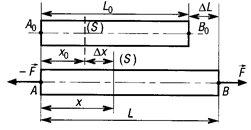
\includegraphics[width=2.61458in,height=1.35417in]{12-RDM/Cours/pandoc/media/image42.png}\ul{Déformations}

Soient~:

\begin{itemize}
\item
  L\textsubscript{0}~: longueur initiale de la poutre (en mm)
\item
  L~: longueur de la poutre après déformation (en mm)
\item
  ∆L~: Allongement de la poutre (en mm)
\item
  ε~:~Allongement relatif de la poutre (sans unité)
\end{itemize}

\begin{quote}
ε = ∆L÷L\textsubscript{0} ou ∆L = ε×L\textsubscript{0}
\end{quote}

\ul{Coefficient de Poisson}

Il traduit un rapport de proportionnalité entre l'allongement longitudinale (ε\textsubscript{L}) et l'allongement transversal (ε\textsubscript{D})

\begin{quote}
ε\textsubscript{D} = -ν×ε\textsubscript{L}
\end{quote}

\emph{ν≈ 0,3 pour l'acier}

\ul{Loi de Hooke}

En déformation élastique, la contrainte σ varie linéairement en fonction de l'allongement relatif ε.

σ = E×ε

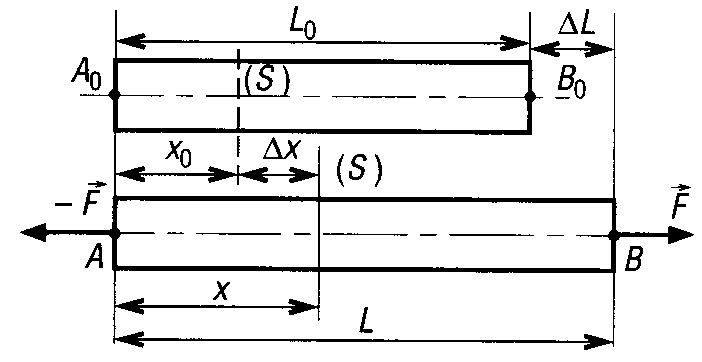
\includegraphics[width=2.60208in,height=1.34236in]{12-RDM/Cours/pandoc/media/image43.png}\emph{E ≈ 210000 MPa pour l'acier}

\begin{longtable}[]{@{}
  >{\raggedright\arraybackslash}p{(\columnwidth - 2\tabcolsep) * \real{0.1111}}
  >{\raggedright\arraybackslash}p{(\columnwidth - 2\tabcolsep) * \real{0.8750}}@{}}
\toprule\noalign{}
\begin{minipage}[b]{\linewidth}\raggedright
\begin{quote}
! \href{12\%20-RDM/\%20Cours\%20/pand\%20oc/me\%20dia/i\%20mage4\%204.png}{}\{wid th=``0 .6262 69685 03937 01in''

heigh t=``0. 65083 33333 33333 4in''\}
\end{quote}
\end{minipage} & \begin{minipage}[b]{\linewidth}\raggedright
\textbf{Tirant}

Un tirant de 2 m de long supporte dans une section droite un effort normal d'extension de N = 5000 N. Il est en acier pour lequel : R\textsubscript{e} = 300 Mpa et E = 200000 Mpa. Déterminer son diamètre minimal Ø et son allongement∆L, en prenant un coefficient de sécurité s = 1,7.
\end{minipage} \\
\midrule\noalign{}
\endhead
\bottomrule\noalign{}
\endlastfoot
& \\
\end{longtable}

\hypertarget{flexion}{%
\subsection{Flexion}\label{flexion}}


\includegraphics{12-RDM/Cours/pandoc/media/image45.emf}\ul{Contrainte normale}

\begin{quote}
\[\sigma = E \times \frac{y}{\rho} = E \times y \times \frac{\Delta\theta}{L_{0}}\]
\end{quote}

\[\sigma = \frac{Mf_{z}}{I_{Gz}} \times y\ ou\text{ M}\text{f}_{z} = \frac{E}{\rho} \times I_{\text{Gz}}\]

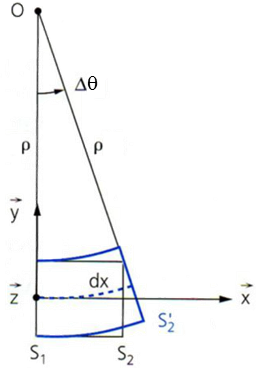
\includegraphics[width=1.70694in,height=2.45347in]{12-RDM/Cours/pandoc/media/image46.png}

\hypertarget{condition-de-ruxe9sistance-1}{%
\subsubsection{Condition de résistance}\label{condition-de-ruxe9sistance-1}}

Soient~:

\begin{itemize}
\item
  K\textsubscript{f} le coefficient de concentration de contrainte~: σ\textsubscript{maxi} = K\textsubscript{f}×σ\textsubscript{moyen}
\item
  R\textsubscript{e} la résistance élastique à l'extension du matériau (en Mpa)
\item
  s un coefficient de sécurité
\item
  R\textsubscript{pe} la résistance pratique à l'extension, avec R\textsubscript{pe} = R\textsubscript{e}÷s
\end{itemize}

Alors, la condition de résistance s'écrit~: σ\textsubscript{maxi}≤R\textsubscript{pe} et/ou f = y\textsubscript{max}≤y\textsubscript{limite} pour les contraintes technologiques

\hypertarget{duxe9formations}{%
\subsubsection{Déformations}\label{duxe9formations}}

\begin{longtable}[]{@{}
  >{\raggedright\arraybackslash}p{(\columnwidth - 6\tabcolsep) * \real{0.2917}}
  >{\raggedright\arraybackslash}p{(\columnwidth - 6\tabcolsep) * \real{0.2778}}
  >{\raggedright\arraybackslash}p{(\columnwidth - 6\tabcolsep) * \real{0.2222}}
  >{\raggedright\arraybackslash}p{(\columnwidth - 6\tabcolsep) * \real{0.1806}}@{}}
\toprule\noalign{}
\begin{minipage}[b]{\linewidth}\raggedright
Equation différentielle de la déformée~:

\[\text{y''} =
 \frac{\text{M}\te
xt{f}_{z}}{E \time
s I_{\text{Gz}}}\]

E~: Module d'Young (en MPa)

I\textsubscript{Gz}~: Moment quadratique (en mm\textsuperscript{4})

Mf\textsubscript{z}~: Moment de flexion (en Nmm)

F~: Effort (N) pour les charges concentrées

F~: Effort linéique (N/mm) pour les charges réparties
\end{minipage} & \begin{minipage}[b]{\linewidth}\raggedright
\textbf{\emph{Disposition des charges}}
\end{minipage} & \begin{minipage}[b]{\linewidth}\raggedright
\textbf{\emph{Moment fléchissant Mf (Nm)}}
\end{minipage} & \begin{minipage}[b]{\linewidth}\raggedright
\textbf{\emph{Flèche maxi f (mm)}}
\end{minipage} \\
\midrule\noalign{}
\endhead
\bottomrule\noalign{}
\endlastfoot
& 
\includegraphics{12-R DM/Cours/pandoc/m edia/image47.png}

\emph{Poutre sur 2 appuis} & {[}{]} (12-RDM/Cours /pandoc/media /image48.wmf) & \includegraphics{12-RDM/C ours/pando c/media/im age49.wmf} \\
& 
\includegraphics{12-R DM/Cours/pandoc/m edia/image50.png} & {[}{]} (12-RDM/Cours /pandoc/media /image51.wmf) & \includegraphics{12-RDM/C ours/pando c/media/im age52.wmf} \\
& 
\includegraphics{12-R DM/Cours/pandoc/m edia/image53.png}

\emph{Poutre encastrée} & {[}{]} (12-RDM/Cours /pandoc/media /image54.wmf) & \includegraphics{12-RDM/C ours/pando c/media/im age55.wmf} \\
& 
\includegraphics{12-R DM/Cours/pandoc/m edia/image56.png} & {[}{]} (12-RDM/Cours /pandoc/media /image57.wmf) & \includegraphics{12-RDM/C ours/pando c/media/im age58.wmf} \\
\end{longtable}

\hypertarget{sources}{%
\subsection{Sources}\label{sources}}

Ce cours a été élaboré à l'aide de nombreuses ressources~provenant de documents publics d'industriels, des activités pédagogiques de collègues de l'UPSTI.

\hypertarget{exercices-du-chapitre}{%
\subsection{Exercices du chapitre}\label{exercices-du-chapitre}}


\includegraphics[width=5.46667in,height=8.37353in]{12-RDM/Cours/pandoc/media/image59.png}


\includegraphics[width=1.35556in,height=0.38889in]{12-RDM/Cours/pandoc/media/image60.png}\textbf{TRACTION - COMPRESSION}

\emph{(\ul{Source} : Jérôme Letard)}

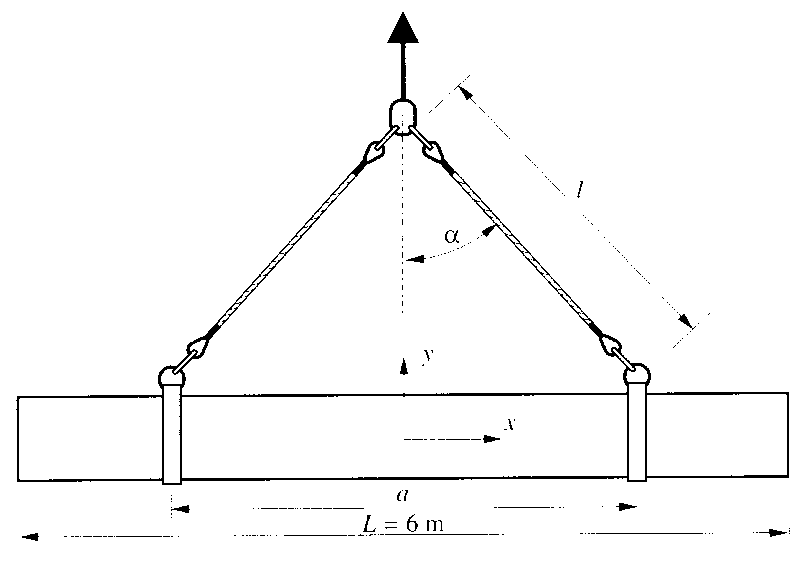
\includegraphics[width=3.67153in,height=2.43333in]{12-RDM/Cours/pandoc/media/image61.png}\textbf{Exercice 1~: Choix d'un câble}

On se propose de soulever une poutre de béton armé de 6 m de longueur et dont la masse est de 2 tonnes.

Pour cela, on dispose symétriquement de deux sangles séparées d'une distance a. Chaque sangle comporte un anneau sur lequel on ancre les crochets d'une élingue formée de deux brins de câble de longueur l = 4 m chacun.

Le câble de diamètre d est constitué de six torons de 19 fils de diamètre d = 0,8 mm chacun et d'une âme textile(AT) dont on néglige la résistance mécanique.

\textbf{1.} Déterminer la tension maximale dans un câble.

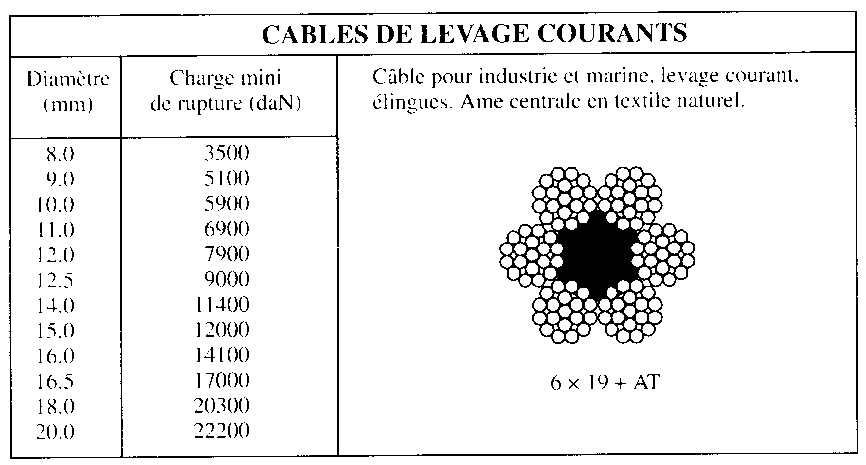
\includegraphics[width=3.93542in,height=2.11042in]{12-RDM/Cours/pandoc/media/image62.png}\textbf{2.} Le coefficient de sécurité étant s = 6 pour les structures de levage, en déduire le diamètre du câble à choisir.

\textbf{3.} La contrainte limite élastique d'un fil est : R\textsubscript{e} = 1770 N/mm². Déterminer le coefficient de sécurité effectif

\textbf{Exercice 2~: Câble de puits de mine}

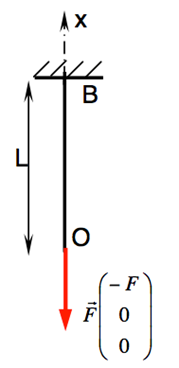
\includegraphics[width=1.19375in,height=2.45347in]{12-RDM/Cours/pandoc/media/image63.png}\ul{Objectif~:} Déterminer la forme d'égale résistance d'un câble soumis à son propre poids et supportant une nacelle de F = 2.10\textsuperscript{3}daNen son extrémité.

\ul{Caractéristiques du câble~:}

Poids volumique : ω =7,8 daN/dm\textsuperscript{3}

Matière~: acier, d'où une contrainte admissible : R\textsubscript{pe}=100MPa

Longueur L = 500 m

\ul{Questions~:}

\textbf{1.} Soit un câble de diamètre Ø variable (pour obtenir la même contrainte dans toutes les sections). On montre alors que la section s'exprime par 
\includegraphics{12-RDM/Cours/pandoc/media/image64.wmf}. Déterminer les diamètres extrêmes du câble.

\textbf{2.} Soit un câble de section constante. Déterminer le diamètre du câble supportant la même nacelle.

\textbf{3.} Calculer la masse respective des 2 câbles précédents.

\textbf{Exercice 3~: Bielle moteur}

\ul{Compression}

Une bielle de moteur diesel est soumise à un effort maximal de compression de 150.10\textsuperscript{3} N. La partie centrale de cette bielle est modélisée par un prisme de section S=300 mm² et de longueur L = 180 mm.

\textbf{1.} Si on adopte un coefficient de sécurité s = 1,2 quelle doit être la limite R\textsubscript{e} de l'acier spécial utilisé ?

\textbf{2.} Si le module d'élasticité longitudinale de cet acier vaut E = 2.10\textsuperscript{5}MPa, quel est le raccourcissement de cette bielle lors de la valeur maximale de l'effort de compression ?

\ul{Parois minces}

Le moteur diesel a un piston de diamètre d = 155 mm et il règne dans la chambre d'explosion une pression effective p=8MPa. La chemise du cylindre est un tube (longueur L, diamètre intérieur d et épaisseur e) en fonte spéciale pour laquelle la contrainte pratique à l'extension peut être prise égale à R\textsubscript{pe} = 50 MPa. On admettra que l'épaisseur de la paroi de la chemise est faible devant son diamètre intérieur d.

A l'intérieur de ce tube règne une pression p\textsubscript{i}.

Soit S la surface hachurée du tube.

L'effort normal est défini par N = p×L×d avec p = p\textsubscript{i} -- p\textsubscript{atm}.

\textbf{3.} Calculer l'épaisseur à donner à la chemise.

\textbf{Exercice 4~: Maillon de chaîne}

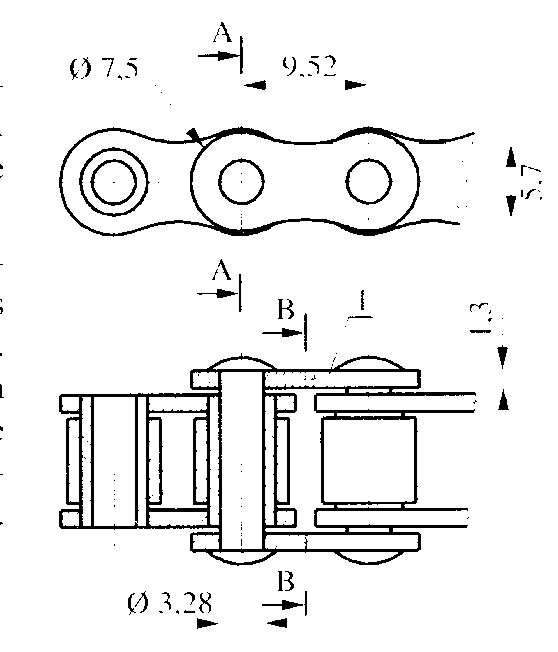
\includegraphics[width=2.39583in,height=2.96181in]{12-RDM/Cours/pandoc/media/image65.png}\ul{Mise en situation}

La figure ci-contre représente une chaîne à rouleaux destinée à transmettre une puissance rotative entre deux arbres parallèles. On se propose d'étudier la résistance de la plaquette 1 à la sollicitation de traction.

Le perçage situé dans le plan de coupe A-A engendre, dans la plaquette étudiée, une concentration de contraintes normales caractérisée par le coefficient K\textsubscript{tp} = 1,6.

De même, on associe le coefficient K\textsubscript{tr} = 1,05 à la réduction de la section située au niveau du plan de coupe B.

L'acier qui constitue la pièce 1 a pour caractéristiques :

R\textsubscript{m} = 1300 MPa, R\textsubscript{e} = 1100 MPa, E = 2,2.10\textsuperscript{5} MPa.

\ul{Questions}

\textbf{1.} Evaluer F\textsubscript{lim}, charge de limite à la rupture de la chaîne en traction statique.

\textbf{2.} En fonctionnement dynamique, dans une application particulière, on impose un coefficient de sécurité s = 3. Quelle est alors la charge maximale en service F\textsubscript{max}~?


\includegraphics[width=1.35556in,height=0.38889in]{12-RDM/Cours/pandoc/media/image60.png} \textbf{FARDELEUSE}

\emph{(\ul{Source} : CCPTSI 2011)}

*Etude des roulements menée en TSI1

\textbf{Mise en situation}

\begin{figure}
\centering
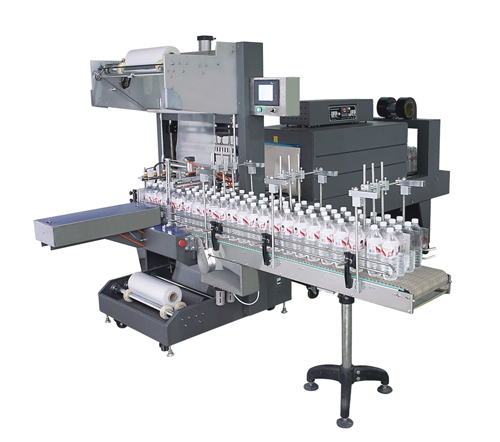
\includegraphics[width=3.25486in,height=2.5in]{12-RDM/Cours/pandoc/media/image66.jpeg}
\caption{http://www.benelite.com/v2/site/images/annonces/FAD-250.jpg}
\end{figure}

Le fardelage consiste à déposer un film plastique thermo-rétractable puis à le chauffer pour qu'il épouse la forme du produit à emballer. Cette opération est réalisée sur la fardeleuse ci-contre

Le produit à fardeler est convoyé par l'ensemble de motorisation ci-dessous

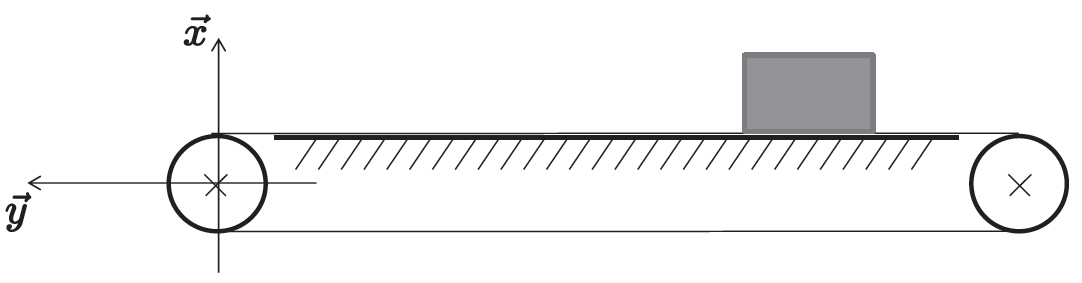
\includegraphics[width=3.90566in,height=1.021in]{12-RDM/Cours/pandoc/media/image67.png}

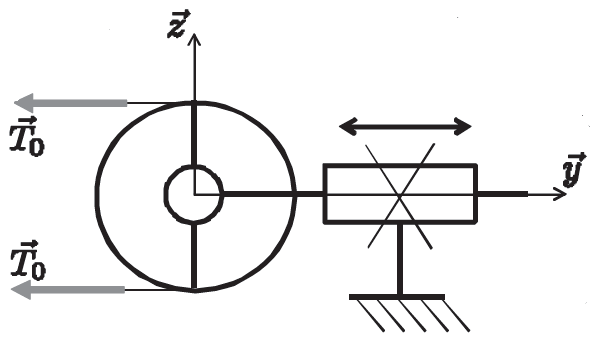
\includegraphics[width=2.58819in,height=1.49028in]{12-RDM/Cours/pandoc/media/image68.png}

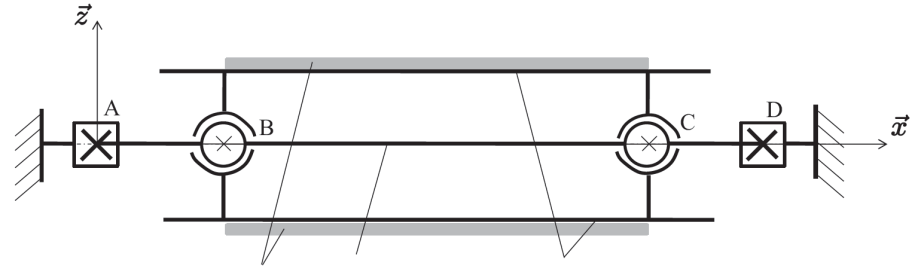
\includegraphics[width=4.16944in,height=1.22361in]{12-RDM/Cours/pandoc/media/image69.png}Le tapis est entrainé par deux cylindres : le cylindre moteur et le cylindre tendeur. Le tapis est entrainé par adhérence. Pour que la transmission de puissance se fasse sans glissement, le tapis doitêtre tendu. A l'arrêt, la tension \textbf{T\textsubscript{0}} est réglée en translatant l'axe du cylindre tendeur.

On considérera que le tapis est positionné symétriquement sur chaque cylindre.

Le cylindre tendeurest guidé en rotation par rapport à l'axe lié au bâti par deux roulements en B et C. L'ensemblepouvant se déplacer par rapport au bâti pour tendre le tapis.

\textbf{Dimensionnement de l'axe de la liaison pivot}

L'axe permettant de guider en rotation le cylindre récepteur est soumis à des actions mécaniques.

On cherche tout d'abord à le dimensionner. L'axe sera considéré cylindrique de diamètre d.~On retient le modèle poutre et les conditions limites suivantes pour l'axe :

Conditions limites sur l'axe

On suppose que l'axe est sur deux appuis en A et D et que les deux roulements exercent deux efforts en B et C :

\(\overrightarrow{F}\) = -F.y avec F = 230 N.

\textbf{1.} Donner la relation entre \textbf{T\textsubscript{0}}, la tension du tapis et \textbf{F}, la norme des efforts en B et C.

\textbf{2.} Donner la résultante des efforts aux appuis en A et D sur l'axe en fonction de \textbf{F}.

\textbf{3.} Exprimer les composantes du torseur de cohésion le long de la poutre et tracer les diagrammes correspondants. A quelle sollicitation est soumise la poutre ?

\textbf{4.} En négligeant l'effort tranchant T\textsubscript{y}, quelle zone de la poutre est la plus sollicitée ?

\textbf{5.} Déterminer la contrainte maximale dans la poutre \(\sigma_{{xx}_{\max}}\)

Pour dimensionner l'axe, on souhaite que la contrainte normale soit inférieure à la limite élastique R\textsubscript{e}, corrigée d'un coefficient de sécurité S\textsubscript{c} supérieur à 1. On considérera S\textsubscript{c} = 2.

\textbf{6.} Donner l'expression du diamètre minimal d\textsubscript{mini} respectant le critère de dimensionnement.

\textbf{Choix d'un matériau pour l'axe de la liaison pivot}

Pour l'axe, il a été choisi d'acheter des barres cylindriques chez un métallurgiste. Il existe des barres avec des diamètres de 3 mm à 50 mm. On donne dans le tableau suivant les différents aciers possibles pour l'axe de la liaison pivot.

\begin{longtable}[]{@{}
  >{\raggedright\arraybackslash}p{(\columnwidth - 6\tabcolsep) * \real{0.2133}}
  >{\raggedright\arraybackslash}p{(\columnwidth - 6\tabcolsep) * \real{0.3333}}
  >{\raggedright\arraybackslash}p{(\columnwidth - 6\tabcolsep) * \real{0.2133}}
  >{\raggedright\arraybackslash}p{(\columnwidth - 6\tabcolsep) * \real{0.2133}}@{}}
\toprule\noalign{}
\begin{minipage}[b]{\linewidth}\raggedright
Acier
\end{minipage} & \begin{minipage}[b]{\linewidth}\raggedright
Etat
\end{minipage} & \begin{minipage}[b]{\linewidth}\raggedright
R\textsubscript{e} en MPa
\end{minipage} & \begin{minipage}[b]{\linewidth}\raggedright
R\textsubscript{m} en MPa
\end{minipage} \\
\midrule\noalign{}
\endhead
\bottomrule\noalign{}
\endlastfoot
C22 & Normalisé & 240 & 430 \\
& Trempé et revenu & 340 & 650 \\
C55 & Normalisé & 370 & 680 \\
& Trempé et revenu & 550 & 950 \\
15 Cr Ni 6 & Trempé et revenu & 650 & 1000 \\
25 Cr Mo 4 & Trempé et revenu & 550 & 850 \\
\end{longtable}

\textbf{7.} Parmi les aciers proposés ci-dessus, choisir l'acier et l'état de cet acier qui pourraient convenir pour l'application étudiée.

\textbf{8.} Pour l'acier choisi, déterminer la valeur de d\textsubscript{mini}.

\textbf{\ul{QUESTIONS DE COURS}}

\textbf{Soin :} \emph{\ldots\ldots{} \textbf{(2 points)}}

\begin{enumerate}
\def\labelenumi{\arabic{enumi}.}
\item
  Citer les deux principaux objectifs d'une étude de RdM. Préciser cet acronyme. \textbf{\emph{(1 point)}}
\item
  Donner (sans les décrire) les 5 principales hypothèses qui permettent de simplifier le modèle d'une étude de RdM. \textbf{\emph{(2,5 points)}}
\item
  Ecrire le torseur de cohésion. Préciser le nom de ses 6 composantes. \textbf{\emph{(2 points)}}
\item
  Donnerl'expression du vecteur contrainte 
\includegraphics{12-RDM/Cours/pandoc/media/image71.wmf}. \textbf{\emph{(0,5 point)}}
\item
  Donner la condition de résistance d'une pièce soumise à de la traction. Préciser les différents termes utilisés. \textbf{\emph{(1,5 point)}}
\item
  Citer 6 sollicitations simples. \textbf{\emph{(1,5 point)}}
\item
  Donner les deux lois de Hooke. Préciser le nom des modules ainsi que la relation entre ces deux modules. \textbf{\emph{(2 points)}}
\item
  Compléter le tableau ci-dessous. \textbf{\emph{(2 points)}}
\end{enumerate}

\begin{longtable}[]{@{}
  >{\raggedright\arraybackslash}p{(\columnwidth - 16\tabcolsep) * \real{0.1359}}
  >{\raggedright\arraybackslash}p{(\columnwidth - 16\tabcolsep) * \real{0.1359}}
  >{\raggedright\arraybackslash}p{(\columnwidth - 16\tabcolsep) * \real{0.0874}}
  >{\raggedright\arraybackslash}p{(\columnwidth - 16\tabcolsep) * \real{0.0971}}
  >{\raggedright\arraybackslash}p{(\columnwidth - 16\tabcolsep) * \real{0.1262}}
  >{\raggedright\arraybackslash}p{(\columnwidth - 16\tabcolsep) * \real{0.0777}}
  >{\raggedright\arraybackslash}p{(\columnwidth - 16\tabcolsep) * \real{0.1456}}
  >{\raggedright\arraybackslash}p{(\columnwidth - 16\tabcolsep) * \real{0.0777}}
  >{\raggedright\arraybackslash}p{(\columnwidth - 16\tabcolsep) * \real{0.0971}}@{}}
\toprule\noalign{}
\begin{minipage}[b]{\linewidth}\raggedright
Lettre grec
\end{minipage} & \begin{minipage}[b]{\linewidth}\raggedright
\end{minipage} & \begin{minipage}[b]{\linewidth}\raggedright
θ
\end{minipage} & \begin{minipage}[b]{\linewidth}\raggedright
\end{minipage} & \begin{minipage}[b]{\linewidth}\raggedright
\end{minipage} & \begin{minipage}[b]{\linewidth}\raggedright
\end{minipage} & \begin{minipage}[b]{\linewidth}\raggedright
\end{minipage} & \begin{minipage}[b]{\linewidth}\raggedright
γ
\end{minipage} & \begin{minipage}[b]{\linewidth}\raggedright
\end{minipage} \\
\midrule\noalign{}
\endhead
\bottomrule\noalign{}
\endlastfoot
Nom & & & epsilon & & rhô & & & \\
Utilisation en RdM & Coefficient de Poisson & & & Contrainte normale & & Contrainte tangentielle & & Angle de torsion \\
\end{longtable}

\begin{enumerate}
\def\labelenumi{\arabic{enumi}.}
\setcounter{enumi}{8}
\tightlist
\item
  Relier correctement (en faisant preuve de logique). \textbf{\emph{(1 point)}}
\end{enumerate}

\begin{longtable}[]{@{}l@{}}
\toprule\noalign{}
\endhead
\bottomrule\noalign{}
\endlastfoot
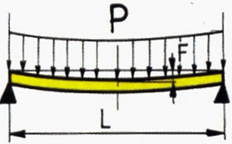
\includegraphics{12-RDM/Cours/pandoc/media/image72.png} 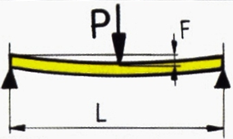
\includegraphics{12-RDM/Cours/pandoc/media/image73.png} 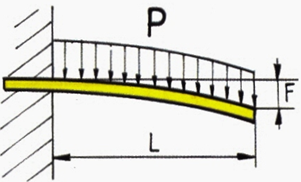
\includegraphics{12-RDM/Cours/pandoc/media/image74.png} 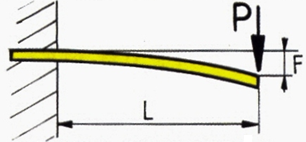
\includegraphics{12-RDM/Cours/pandoc/media/image75.png} \\
\end{longtable}


\includegraphics{12-RDM/Cours/pandoc/media/image76.wmf} 
\includegraphics{12-RDM/Cours/pandoc/media/image77.wmf} 
\includegraphics{12-RDM/Cours/pandoc/media/image78.wmf} 
\includegraphics{12-RDM/Cours/pandoc/media/image79.wmf} -----------------------------------------------------------------------------------------------------------------------------------------------------------------------------------

\begin{enumerate}
\def\labelenumi{\arabic{enumi}.}
\setcounter{enumi}{9}
\item
  Comment s'appelle F~? \textbf{\emph{(0,5 point)}}
\item
  Donner l'expression de σ pour les deux sollicitations suivantes. \textbf{\emph{(2 points)}}
\item
  Donner le nom et les unités des grandeurs suivantes. \textbf{\emph{(1 point)}}
\end{enumerate}

\begin{longtable}[]{@{}
  >{\raggedright\arraybackslash}p{(\columnwidth - 8\tabcolsep) * \real{0.1282}}
  >{\raggedright\arraybackslash}p{(\columnwidth - 8\tabcolsep) * \real{0.1923}}
  >{\raggedright\arraybackslash}p{(\columnwidth - 8\tabcolsep) * \real{0.1923}}
  >{\raggedright\arraybackslash}p{(\columnwidth - 8\tabcolsep) * \real{0.2179}}
  >{\raggedright\arraybackslash}p{(\columnwidth - 8\tabcolsep) * \real{0.2436}}@{}}
\toprule\noalign{}
\begin{minipage}[b]{\linewidth}\raggedright
Symbole
\end{minipage} & \begin{minipage}[b]{\linewidth}\raggedright
I\textsubscript{Gz}
\end{minipage} & \begin{minipage}[b]{\linewidth}\raggedright
y'
\end{minipage} & \begin{minipage}[b]{\linewidth}\raggedright
Mf\textsubscript{z}
\end{minipage} & \begin{minipage}[b]{\linewidth}\raggedright
R\textsubscript{pe}
\end{minipage} \\
\midrule\noalign{}
\endhead
\bottomrule\noalign{}
\endlastfoot
Nom & & & & \\
Unité & & & & \\
\end{longtable}

\begin{enumerate}
\def\labelenumi{\arabic{enumi}.}
\setcounter{enumi}{12}
\item
  Donner l'équation différentielle de la déformée en flexion. \textbf{\emph{(1 point)}}
\item
  Pour les cas suivants, donner les conditions aux limites pour trouver les constantes d'intégration. \textbf{\emph{(1,5 point)}}
\end{enumerate}

\begin{longtable}[]{@{}
  >{\raggedright\arraybackslash}p{(\columnwidth - 6\tabcolsep) * \real{0.2329}}
  >{\raggedright\arraybackslash}p{(\columnwidth - 6\tabcolsep) * \real{0.2466}}
  >{\raggedright\arraybackslash}p{(\columnwidth - 6\tabcolsep) * \real{0.2466}}
  >{\raggedright\arraybackslash}p{(\columnwidth - 6\tabcolsep) * \real{0.2466}}@{}}
\toprule\noalign{}
\begin{minipage}[b]{\linewidth}\raggedright
\end{minipage} & \begin{minipage}[b]{\linewidth}\raggedright
\end{minipage} & \begin{minipage}[b]{\linewidth}\raggedright
\end{minipage} & \begin{minipage}[b]{\linewidth}\raggedright
Condition de continuité en un point
\end{minipage} \\
\midrule\noalign{}
\endhead
\bottomrule\noalign{}
\endlastfoot
y(x=0) =

y'(x=0) = & y(x=a) = & y\textquotesingle(x=a) = & y\textsubscript{1}(x=a) =

y'\textsubscript{1}(x=a) = \\
\end{longtable}

\textbf{\ul{EXERCICE~: DEFAUTS ET AUTOCONTRAINTES}}

L'arbre (2) est lié au carter (1) par l'intermédiaire de deux roulements.

Le premier, en O\textsubscript{1} est un roulement à double rangée de billes à contacts obliques dont les deux bagues sont arrêtées axialement. Il est modélisé par une liaison pivot d'axe x\textsubscript{1}.

Le second, en A, est un roulement à billes à contact radial dont la bague extérieure est libre en translation. Il est modélisé par une liaison linéaire annulaire.

Après fabrication, on constate sur le carter (1) un défaut de coaxialité entre les alésages qui reçoivent les bagues extérieures des deux roulements. Ce défaut est caractérisé par δ\textsubscript{r} sur le schéma qui suit. Au montage, ce défaut va engendrer des efforts au niveau des liaisons et des autocontraintes dans l'arbre.

L'exercice consiste à chiffrer ces divers effets sur ce montage de roulements.

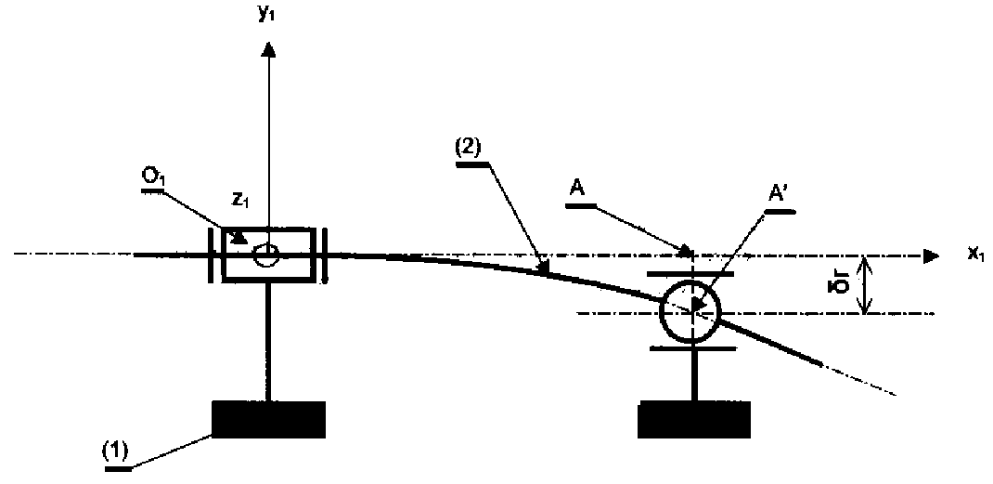
\includegraphics[width=4.48333in,height=2.18337in]{12-RDM/Cours/pandoc/media/image80.png}

\textbf{1.} On considère que le problème de mécanique est plan. L'axe y\textsubscript{1} est choisi tel que z\textsubscript{A'} = 0. On note X\textsubscript{O}, Y\textsubscript{O} \ldots{} N\textsubscript{O} \ldots{} Y\textsubscript{A} les composantes du torseur des actions de liaison du bâti sur l'arbre en O\textsubscript{1} et A.

\textbf{a.} En considérant le problème plan (en «~2D~»), écrire les torseurs des inconnues de liaisons aux points O\textsubscript{1} et A. \textbf{\emph{(2 points)}}

\textbf{b.} Faire le bilan des inconnues de liaisons et en déduire le rang du système d'équations issu du PFS (ordre d'hyperstatisme interne) de cette liaison pivot entre arbre et carter. \textbf{\emph{(1 point)}}

\textbf{c.} Aucune charge extérieure n'agit sur l'arbre. En appliquant le PFS, déterminer les 3 relations qui relient les inconnues de liaison. \textbf{\emph{(3 points)}}

\textbf{2.} La section de l'arbre a un moment quadratique I\textsubscript{Gz} et son matériau un module d'Young E

\textbf{a.} Montrer que l'expression littérale du moment fléchissant Mf\textsubscript{z} en fonction de x et des inconnues de la liaison en O\textsubscript{1} est Mf\textsubscript{z} = -N\textsubscript{O} + x×Y\textsubscript{O}. \textbf{\emph{(2 points)}}

\textbf{b.} En utilisant les deux conditions aux limites au point O\textsubscript{1}, déterminer l'expression littérale de la déformée y(x) en fonction des caractéristiques de l'arbre et des inconnues de la liaison en O\textsubscript{1}. \textbf{\emph{(3 points)}}

\textbf{c.} En utilisant la condition aux limites au point A (pour lever l'hyperstaticité établie précédemment), montrer que \(Y_{A} = \frac{3.E.I_{Gz}.\delta_{r}}{L^{3}}\). Déterminer alors l'expression littérale des inconnues de la liaison en O\textsubscript{1} en fonction des caractéristiques de l'arbre et du défaut δ\textsubscript{r}. \textbf{\emph{(2 points)}}

\textbf{d.} En déduire l'expression littérale de la déformée y(x) en fonction des caractéristiques de l'arbre et du défaut δ\textsubscript{r}. \textbf{\emph{(0 point)}}

\textbf{3.} L'arbre a un diamètre de 20 mm~; L = 300 mm~; E = 2.10\textsuperscript{5}MPa et δ\textsubscript{r} = 0,05 mm.

\textbf{a.} Calculer le moment quadratique I\textsubscript{Gz}= \(\frac{\pi D^{4}}{64}\).\textbf{\emph{(1 point)}}

\textbf{b.} Calculer les actions de liaison. \textbf{\emph{(2 point)}}

\textbf{c.} Calculer le moment fléchissant maximal Mf\textsubscript{zmaxi} puis l'autocontrainte normale maximale σ\textsubscript{maxi} dans l'arbre. \textbf{\emph{(2 points)}}

\textbf{\ul{QCM}}

Une seule réponse / question. Noircir la bonne réponse. Pour toutes les AN, π = 3 et g = 10 m/s²

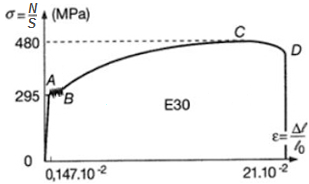
\includegraphics[width=3.21667in,height=1.91528in]{12-RDM/Cours/pandoc/media/image81.png}+1 / bonne réponse -0,5 / mauvaise réponse 0 sans réponse

\begin{enumerate}
\def\labelenumi{\arabic{enumi}.}
\tightlist
\item
  Comment s'appelle ce diagramme~?
\end{enumerate}

\begin{longtable}[]{@{}l@{}}
\toprule\noalign{}
\endhead
\bottomrule\noalign{}
\endlastfoot
Hooke Traction Elasticité Contrainte-déformation Young \\
\end{longtable}

\begin{center}\rule{0.5\linewidth}{0.5pt}\end{center}

\begin{enumerate}
\def\labelenumi{\arabic{enumi}.}
\setcounter{enumi}{1}
\tightlist
\item
  Quelle est la zone entre A et B~?
\end{enumerate}

\begin{longtable}[]{@{}l@{}}
\toprule\noalign{}
\endhead
\bottomrule\noalign{}
\endlastfoot
Elastique Rupture Striction Plastique Ecrouissage \\
\end{longtable}

\begin{center}\rule{0.5\linewidth}{0.5pt}\end{center}

\begin{enumerate}
\def\labelenumi{\arabic{enumi}.}
\setcounter{enumi}{2}
\tightlist
\item
  Quelle est la bonne réponse sur la caractéristique de l'acier E30~?
\end{enumerate}

\(\varepsilon = \frac{\mathcal{\mathrm{\Delta}l}}{\mathcal{l}_{0}}\) est l\textquotesingle allongement en \% de la matière

A est la limite à la rupture Entre B et C, σ = E×ε

C est l\textquotesingle allongement maximum σ est une contrainte de cisaillement

Au-delà de 295 N/m² les déformations sont permanentes

\begin{enumerate}
\def\labelenumi{\arabic{enumi}.}
\setcounter{enumi}{3}
\tightlist
\item
  Quelle est la valeur du module d'Young (GPa) du plexiglas~?
\end{enumerate}

\begin{longtable}[]{@{}l@{}}
\toprule\noalign{}
\endhead
\bottomrule\noalign{}
\endlastfoot
62 3,1 80 à 130 11 à 13 210 \\
\end{longtable}

\begin{center}\rule{0.5\linewidth}{0.5pt}\end{center}

\begin{enumerate}
\def\labelenumi{\arabic{enumi}.}
\setcounter{enumi}{4}
\tightlist
\item
  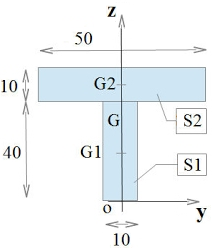
\includegraphics[width=2.20755in,height=2.58491in]{12-RDM/Cours/pandoc/media/image82.png}Quelle est la coordonnée z\textsubscript{G} du centre de la surface \{S1+S2\}~?
\end{enumerate}

\begin{longtable}[]{@{}l@{}}
\toprule\noalign{}
\endhead
\bottomrule\noalign{}
\endlastfoot
0 20 25 32,5 33,9 40 45 \\
\end{longtable}

\begin{center}\rule{0.5\linewidth}{0.5pt}\end{center}

\begin{enumerate}
\def\labelenumi{\arabic{enumi}.}
\setcounter{enumi}{5}
\tightlist
\item
  Quelle est la mauvaise réponse sur le torseur de cohésion~?
\end{enumerate}

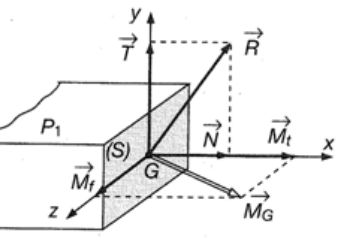
\includegraphics[width=2.45278in,height=1.72708in]{12-RDM/Cours/pandoc/media/image83.png} M\textsubscript{f} veut dire moment fléchissant

Le repère du torseur de cohésion est toujours le même que celui du système étudié

L\textquotesingle effort tranchant sur \(\overrightarrow{z}\) est noté T\textsubscript{Z}

L\textquotesingle effort tranchant sur \(\overrightarrow{y}\) est noté N

M\textsubscript{t} veut dire moment de torsion

Les composantes du torseur de cohésion sont les efforts de la partie de poutre enlevée sur la partie de poutre dont on étudie l\textquotesingle équilibre

\begin{enumerate}
\def\labelenumi{\arabic{enumi}.}
\setcounter{enumi}{6}
\tightlist
\item
  Une poutre de section carrée est soumise au torseur de cohésion . C'est une sollicitation de~?
\end{enumerate}

\begin{longtable}[]{@{}l@{}}
\toprule\noalign{}
\endhead
\bottomrule\noalign{}
\endlastfoot
Traction Compression Cisaillement Torsion Flexion pure Flexion simple \\
\end{longtable}

\begin{center}\rule{0.5\linewidth}{0.5pt}\end{center}

\begin{enumerate}
\def\labelenumi{\arabic{enumi}.}
\setcounter{enumi}{7}
\tightlist
\item
  Quel est l'intrus~?
\end{enumerate}

\begin{longtable}[]{@{}l@{}}
\toprule\noalign{}
\endhead
\bottomrule\noalign{}
\endlastfoot
Résistance Module de Contrainte Moment Pression Limite \\
mécanique Coulomb tangentielle fléchissant uniforme pratique au \\
glissement \\
\end{longtable}

\begin{center}\rule{0.5\linewidth}{0.5pt}\end{center}

\begin{enumerate}
\def\labelenumi{\arabic{enumi}.}
\setcounter{enumi}{8}
\tightlist
\item
  Dans un torseur de cohésion, que représente N~?
\end{enumerate}

\begin{longtable}[]{@{}l@{}}
\toprule\noalign{}
\endhead
\bottomrule\noalign{}
\endlastfoot
Effort Newton Moment Effort Moment net Effort \\
naturel nominal national normal \\
\end{longtable}

\begin{center}\rule{0.5\linewidth}{0.5pt}\end{center}

\begin{enumerate}
\def\labelenumi{\arabic{enumi}.}
\setcounter{enumi}{9}
\tightlist
\item
  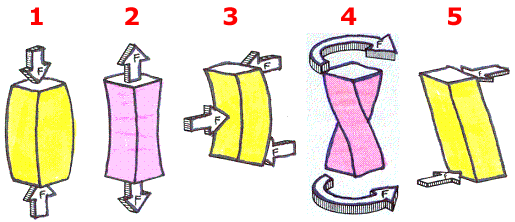
\includegraphics[width=3.30139in,height=1.34861in]{12-RDM/Cours/pandoc/media/image84.png}A quelle sollicitation est soumise la pièce n°4~?
\end{enumerate}

\begin{longtable}[]{@{}l@{}}
\toprule\noalign{}
\endhead
\bottomrule\noalign{}
\endlastfoot
Cisaillement Traction Compression Flexion Torsion \\
\end{longtable}

\begin{center}\rule{0.5\linewidth}{0.5pt}\end{center}

\begin{enumerate}
\def\labelenumi{\arabic{enumi}.}
\setcounter{enumi}{10}
\tightlist
\item
  Quel torseur correspond à la déformation n~2~?
\end{enumerate}

\begin{longtable}[]{@{}l@{}}
\toprule\noalign{}
\endhead
\bottomrule\noalign{}
\endlastfoot
\(\left\{ \begin{array}{r}              \)\left\{ \textbackslash begin\{array\}\{r\} \(\left\{ \begin{array}{r}              \)\left\{ \textbackslash begin\{array\}\{r\} \(\left\{ \begin{array}{r}              \)\left\{ \textbackslash begin\{array\}\{r\} \\
N \textbackslash{} 0 \textbackslash{} 0 \textbackslash{} 0 \textbackslash{} 0 \textbackslash{} 0 \textbackslash{} \\
0 \textbackslash{} T\_\{y\} \textbackslash{} 0 \textbackslash{} 0 \textbackslash{} T\_\{y\} \textbackslash{} 0 \textbackslash{} \\
0 0 0 0 T\_\{z\} 0 \\
\textbackslash end\{array\} \middle\textbar{} \\
0 \textbackslash{} 0 \textbackslash{} 0 \textbackslash{} Mt \textbackslash{} 0 \textbackslash{} 0 \textbackslash{} \\
0 \textbackslash{} 0 \textbackslash{} 0 \textbackslash{} 0 \textbackslash{} 0 \textbackslash{} \{Mf\}\_\{y\} \textbackslash{} \\
0 \{Mf\}\emph{\{z\} \{Mf\}}\{z\} 0 0 \{Mf\}\_\{z\} \\
\textbackslash end\{array\} \right\}\emph{\{G,R\}\(            \end{array} \right\}_{G,R}\) \textbackslash end\{array\} \right\}}\{G,R\}\(            \end{array} \right\}_{G,R}\) \textbackslash end\{array\} \right\}\_\{G,R\}\(            \end{array} \right\}_{G,R}\) \\
\end{longtable}

\begin{center}\rule{0.5\linewidth}{0.5pt}\end{center}

\begin{enumerate}
\def\labelenumi{\arabic{enumi}.}
\setcounter{enumi}{11}
\tightlist
\item
  En quelle unité est exprimé le moment polaire~?
\end{enumerate}

\begin{longtable}[]{@{}l@{}}
\toprule\noalign{}
\endhead
\bottomrule\noalign{}
\endlastfoot
mm N/m\textsuperscript{2} mm\textsuperscript{3} N/mm\textsuperscript{2} MPa mm\textsuperscript{4} Pa mm\textsuperscript{2} \\
\end{longtable}

\begin{center}\rule{0.5\linewidth}{0.5pt}\end{center}

\begin{enumerate}
\def\labelenumi{\arabic{enumi}.}
\setcounter{enumi}{12}
\tightlist
\item
  Combien vaut la déformation relative d'un matériau possédant module d'Young de 40 GPa et recevant sur une surface de 260 mm² une force de 52 kN~?
\end{enumerate}

\begin{longtable}[]{@{}l@{}}
\toprule\noalign{}
\endhead
\bottomrule\noalign{}
\endlastfoot
0,3 \% 0,5 \% 1,5 \% 2 \% \\
\end{longtable}

\begin{center}\rule{0.5\linewidth}{0.5pt}\end{center}

\begin{enumerate}
\def\labelenumi{\arabic{enumi}.}
\setcounter{enumi}{13}
\tightlist
\item
  Quelle est la lettre utilisée pour désigner le coefficient de Lamé~?
\end{enumerate}

\begin{longtable}[]{@{}l@{}}
\toprule\noalign{}
\endhead
\bottomrule\noalign{}
\endlastfoot
ν ε λ θ ρ τ γ σ \\
\end{longtable}

\begin{center}\rule{0.5\linewidth}{0.5pt}\end{center}

\begin{enumerate}
\def\labelenumi{\arabic{enumi}.}
\setcounter{enumi}{14}
\tightlist
\item
  Dans une section droite de poutre rectiligne soumise à de la flexion pure, quel est le type de torseur de cohésion~?
\end{enumerate}

\begin{longtable}[]{@{}l@{}}
\toprule\noalign{}
\endhead
\bottomrule\noalign{}
\endlastfoot
Quelconque Nul Couple Glisseur \\
\end{longtable}

\begin{center}\rule{0.5\linewidth}{0.5pt}\end{center}

\begin{enumerate}
\def\labelenumi{\arabic{enumi}.}
\setcounter{enumi}{15}
\tightlist
\item
  Combien vaut la contrainte exercée sur un matériau par une force normale de 48 N répartie uniformément sur une section circulaire de rayon 12 cm~?
\end{enumerate}

\begin{longtable}[]{@{}l@{}}
\toprule\noalign{}
\endhead
\bottomrule\noalign{}
\endlastfoot
120 Pa 1,1 kPa 6,7 kPa 280 kPa \\
\end{longtable}

\begin{center}\rule{0.5\linewidth}{0.5pt}\end{center}

\begin{enumerate}
\def\labelenumi{\arabic{enumi}.}
\setcounter{enumi}{16}
\tightlist
\item
  Une poutre horizontale de longueur \(\mathcal{l}\) dont on néglige le poids propre est encastrée à une extrémité. Elle est chargée en son autre extrémité d'une force concentrée verticale \(\overrightarrow{F}\). Quelle est l'expression du moment de flexion maximum~?
\end{enumerate}

\begin{longtable}[]{@{}l@{}}
\toprule\noalign{}
\endhead
\bottomrule\noalign{}
\endlastfoot
\(\frac{F\mathcal{l}^{2}}{2}\) \(\frac{F\mathcal{l}}{4}\) \(\frac{F\mathcal{l}}{8}\) \(\frac{F\mathcal{l}^{2}}{8}\) \(\frac{F\mathcal{l}}{2}\) \(F\mathcal{l}\) \\
\end{longtable}

\begin{center}\rule{0.5\linewidth}{0.5pt}\end{center}

\begin{enumerate}
\def\labelenumi{\arabic{enumi}.}
\setcounter{enumi}{17}
\tightlist
\item
  Combien vaut la contrainte maximale exercée sur un matériau par un moment de flexion de 75 Nm sur une section circulaire de diamètre 10 cm~?
\end{enumerate}

\begin{longtable}[]{@{}l@{}}
\toprule\noalign{}
\endhead
\bottomrule\noalign{}
\endlastfoot
160 Pa 400 kPa 0,8 MPa 12,8 MPa \\
\end{longtable}

\begin{center}\rule{0.5\linewidth}{0.5pt}\end{center}

\begin{enumerate}
\def\labelenumi{\arabic{enumi}.}
\setcounter{enumi}{18}
\tightlist
\item
  Comment, sur une poutre droite, modélise-t-on le poids propre~?
\end{enumerate}

Par un glisseur réduit au centre de gravité de la poutre

Par la pesanteur

Par une densité linéique de force

Par des moments appliqués aux points d'appui

\begin{enumerate}
\def\labelenumi{\arabic{enumi}.}
\setcounter{enumi}{19}
\tightlist
\item
  Quelle est la sollicitation composée~?
\end{enumerate}

\begin{longtable}[]{@{}l@{}}
\toprule\noalign{}
\endhead
\bottomrule\noalign{}
\endlastfoot
Pelage Extension Flambage Flexion déviée Cisaillement \\
\end{longtable}

\begin{center}\rule{0.5\linewidth}{0.5pt}\end{center}

\begin{enumerate}
\def\labelenumi{\arabic{enumi}.}
\setcounter{enumi}{20}
\tightlist
\item
  Dans un essai de cisaillement, l'effort appliqué à la poutre est parallèle à \(\overrightarrow{y}\). Quelle composante parasite des éléments de réduction du \{T\textsubscript{coh}\} convient-il de négliger~?
\end{enumerate}

\begin{longtable}[]{@{}l@{}}
\toprule\noalign{}
\endhead
\bottomrule\noalign{}
\endlastfoot
N T\textsubscript{y} T\textsubscript{z} Mt Mf\textsubscript{y} Mf\textsubscript{z} \\
\end{longtable}

\begin{center}\rule{0.5\linewidth}{0.5pt}\end{center}

\begin{enumerate}
\def\labelenumi{\arabic{enumi}.}
\setcounter{enumi}{21}
\tightlist
\item
  Combien vaut la contrainte maximale exercée dans une poutre circulaire de rayon 12 mm par un moment de torsion de 9 Nm~?
\end{enumerate}

\begin{longtable}[]{@{}l@{}}
\toprule\noalign{}
\endhead
\bottomrule\noalign{}
\endlastfoot
3,5 kPa 3,5 MPa 6,9 MPa 27,8 MPa \\
\end{longtable}

\begin{center}\rule{0.5\linewidth}{0.5pt}\end{center}

\begin{center}\rule{0.5\linewidth}{0.5pt}\end{center}

\hypertarget{inventaire-des-images}{%
\subsection{Inventaire des images}\label{inventaire-des-images}}

12-RDM/Cours/pandoc/media/image1.png 12-RDM/Cours/pandoc/media/image10.emf 12-RDM/Cours/pandoc/media/image11.emf 12-RDM/Cours/pandoc/media/image12.emf 12-RDM/Cours/pandoc/media/image13.png 12-RDM/Cours/pandoc/media/image14.png 12-RDM/Cours/pandoc/media/image15.png 12-RDM/Cours/pandoc/media/image16.emf 12-RDM/Cours/pandoc/media/image17.png 12-RDM/Cours/pandoc/media/image18.png 12-RDM/Cours/pandoc/media/image19.png 12-RDM/Cours/pandoc/media/image20.png 12-RDM/Cours/pandoc/media/image21.wmf 12-RDM/Cours/pandoc/media/image22.wmf 12-RDM/Cours/pandoc/media/image23.wmf 12-RDM/Cours/pandoc/media/image24.wmf 12-RDM/Cours/pandoc/media/image25.wmf 12-RDM/Cours/pandoc/media/image26.png 12-RDM/Cours/pandoc/media/image27.wmf 12-RDM/Cours/pandoc/media/image28.wmf 12-RDM/Cours/pandoc/media/image29.wmf 12-RDM/Cours/pandoc/media/image3.jpeg 12-RDM/Cours/pandoc/media/image30.wmf 12-RDM/Cours/pandoc/media/image31.wmf 12-RDM/Cours/pandoc/media/image32.wmf 12-RDM/Cours/pandoc/media/image33.wmf 12-RDM/Cours/pandoc/media/image34.wmf 12-RDM/Cours/pandoc/media/image35.wmf 12-RDM/Cours/pandoc/media/image36.wmf 12-RDM/Cours/pandoc/media/image37.wmf 12-RDM/Cours/pandoc/media/image38.emf 12-RDM/Cours/pandoc/media/image39.emf 12-RDM/Cours/pandoc/media/image40.wmf 12-RDM/Cours/pandoc/media/image41.wmf 12-RDM/Cours/pandoc/media/image42.png 12-RDM/Cours/pandoc/media/image43.png 12-RDM/Cours/pandoc/media/image44.png 12-RDM/Cours/pandoc/media/image45.emf 12-RDM/Cours/pandoc/media/image46.png 12-RDM/Cours/pandoc/media/image47.png 12-RDM/Cours/pandoc/media/image48.wmf 12-RDM/Cours/pandoc/media/image49.wmf 12-RDM/Cours/pandoc/media/image5.png 12-RDM/Cours/pandoc/media/image50.png 12-RDM/Cours/pandoc/media/image51.wmf 12-RDM/Cours/pandoc/media/image52.wmf 12-RDM/Cours/pandoc/media/image53.png 12-RDM/Cours/pandoc/media/image54.wmf 12-RDM/Cours/pandoc/media/image55.wmf 12-RDM/Cours/pandoc/media/image56.png 12-RDM/Cours/pandoc/media/image57.wmf 12-RDM/Cours/pandoc/media/image58.wmf 12-RDM/Cours/pandoc/media/image59.png 12-RDM/Cours/pandoc/media/image6.png 12-RDM/Cours/pandoc/media/image60.png 12-RDM/Cours/pandoc/media/image61.png 12-RDM/Cours/pandoc/media/image62.png 12-RDM/Cours/pandoc/media/image63.png 12-RDM/Cours/pandoc/media/image64.wmf 12-RDM/Cours/pandoc/media/image65.png 12-RDM/Cours/pandoc/media/image66.jpeg 12-RDM/Cours/pandoc/media/image67.png 12-RDM/Cours/pandoc/media/image68.png 12-RDM/Cours/pandoc/media/image69.png 12-RDM/Cours/pandoc/media/image7.png 12-RDM/Cours/pandoc/media/image71.wmf 12-RDM/Cours/pandoc/media/image72.png 12-RDM/Cours/pandoc/media/image73.png 12-RDM/Cours/pandoc/media/image74.png 12-RDM/Cours/pandoc/media/image75.png 12-RDM/Cours/pandoc/media/image76.wmf 12-RDM/Cours/pandoc/media/image77.wmf 12-RDM/Cours/pandoc/media/image78.wmf 12-RDM/Cours/pandoc/media/image79.wmf 12-RDM/Cours/pandoc/media/image8.wmf 12-RDM/Cours/pandoc/media/image80.png 12-RDM/Cours/pandoc/media/image81.png 12-RDM/Cours/pandoc/media/image82.png 12-RDM/Cours/pandoc/media/image83.png 12-RDM/Cours/pandoc/media/image84.png 12-RDM/Cours/pandoc/media/image9.emf
